\documentclass[11pt,letterpaper]{article}
\usepackage[utf8]{inputenc}
\usepackage[margin=1in]{geometry}
\usepackage{graphicx}
\usepackage{subcaption}
\usepackage{hyperref}
\usepackage{amsmath}
\usepackage{float}
\linespread{1.1}
\setlength\parindent{0pt}
\setlength{\parskip}{\baselineskip}

\bibliographystyle{elsarticle-num}

\title{Coupled Laser Simulation Updates}
\author{Godwin Duan}
\date{July 2025}

\begin{document}

\maketitle

\section*{Introduction and Goals}
I wish to investigate the behavior of a system of lasers which are coupled to one another. In this project, I model the system as a set of Coupled Lang-Kobayashi Equations. This set of first-order, delay differential equations are solved numerically by a Python program.

\textbf{Goal:} to use this laser model to simulate the behavior of a physical compute reservoir (PRC). We will compare this (simulated) reservoir's ability to perform classification/prediction tasks against a traditional neural network.

\textbf{Motivation:} It is a slow and costly process to build an actual chip of lasers in the cleanroom, so we first verify that a system of lasers can function as a PRC in software before we actually go build it. This simulation process will also give us intuition into how the lasers should be patterned on our chip and how they should be driven/read out for best performance.

In these notes I primarily reference "Semiconductor Lasers: Stability, Instability, and Chaos" by Ohtsubo~\cite{ohtsubo2017semiconductor}, which I have been reading since mid-June.

My code and figures can be found in my GitHub repo: ~\href{https://github.com/godwinduan/lasersim}{https://github.com/godwinduan/lasersim}

\section{July 9-10, 2025}
Began coding the Coupled Lang-Kobayashi Equations.

\subsection{Coupled Lang-Kobayashi Equations}

For a system of n lasers, the differential equations for the field in laser $j$ are given by:

\begin{multline}
\frac{dE_j(t)}{dt} = \frac{1}{2} (1 - i \alpha) (G_j - \gamma) E_j(t) + \frac{\kappa_{jj}}{\tau_{in}} E_j(t - \tau_{jj}) \text{exp}(i \omega_j \tau_{jj}) \\
+ \sum^{n - 1}_{k=0, k\neq j} \frac{\kappa_{jk}}{\tau_{in}} E_k(t - \tau_{jk}) \text{exp}(-i \Delta\omega_{jk} \tau_{jk})
\end{multline}

where  $\kappa_{jk}$ is the coupling strength from k to j,  $\tau_{jk}$ is the time delay from k to j,  and $\Delta\omega_{jk} = \omega_k - \omega_j$.

The first term on the right is increase in field from the laser's own field.
The second term on the right is the self coupling of the laser (has a delay $\tau_{jj}$).
The third term on the right is the coupling from all other lasers.

To code this, we have to break up the above expression for E into a real component $X_j(t)$ and imaginary component $Y_j(t)$ such that $E_j(t) = X_j(t) + i Y_j(t)$.

\begin{multline}
\frac{dE_j(t)}{dt} = \frac{1}{2}  (G_j - \gamma) E_j(t) - i \alpha \frac{1}{2}  (G_j - \gamma) E_j(t) + \frac{\kappa_{jj}}{\tau_{in}} E_j(t - \tau_{jj}) \cos(\omega_j \tau_{jj}) + i \frac{\kappa_{jj}}{\tau_{in}} E_j(t - \tau_{jj}) \sin(\omega_j \tau_{jj}) \\
+ \sum^{n - 1}_{k=0, k\neq j} \frac{\kappa_{jk}}{\tau_{in}} E_k(t - \tau_{jk}) \cos(\Delta\omega_{jk} \tau_{jk}) - i \sum^{n - 1}_{k=0, k\neq j} \frac{\kappa_{jk}}{\tau_{in}} E_k(t - \tau_{jk}) \sin(\Delta\omega_{jk} \tau_{jk})
\end{multline}

After we expand $E$ into $X$ and $Y$ and distribute terms,

\begin{multline}
\frac{dX_j(t)}{dt} = \frac{1}{2}  (G_j - \gamma) (X_j(t) + \alpha Y_j(t)) + \frac{\kappa_{jj}}{\tau_{in}} (X_j(t - \tau_{jj}) \cos(\omega_j \tau_{jj}) - Y_j(t - \tau_{jj}) \sin(\omega_j \tau_{jj})) \\
+ \sum^{n - 1}_{k=0, k\neq j} \frac{\kappa_{jk}}{\tau_{in}} ( X_k(t - \tau_{jk}) \cos(\Delta\omega_{jk} \tau_{jk}) + Y_k(t - \tau_{jk}) \sin(\Delta\omega_{jk} \tau_{jk}))
\end{multline}

\begin{multline}
\frac{dY_j(t)}{dt} = \frac{1}{2}  (G_j - \gamma) (Y_j(t) - \alpha X_j(t)) + \frac{\kappa_{jj}}{\tau_{in}} (Y_j(t - \tau_{jj}) \cos(\omega_j \tau_{jj}) + X_j(t - \tau_{jj}) \sin(\omega_j \tau_{jj})) \\
+ \sum^{n - 1}_{k=0, k\neq j} \frac{\kappa_{jk}}{\tau_{in}} ( Y_k(t - \tau_{jk}) \cos(\Delta\omega_{jk} \tau_{jk}) - X_k(t - \tau_{jk}) \sin(\Delta\omega_{jk} \tau_{jk}))
\end{multline}

For the carrier density of laser $j$,
\begin{equation}
\frac{dN_j(t)}{dt} = \frac{I_j}{e} - \gamma_e * N_j - G_j * |E|^2
\end{equation}

Where $|E|^2 = X^2 + Y^2$, and

\[
G_j = \frac{g(N_j - N_0)}{1 + s |E|^2}
\]

\subsection{Comments}
\begin{itemize}
    \item Question: is it plus alpha or minus alpha in the Lang-Kobayashi Equation? In Ohtsubo's textbook, it is minus (see Ohtsubo 87), and I am following this convention, but in the original Lang-Kobayashi paper (and in Chixuan's work), it is plus alpha. As a result my equations' signs differ from Chixuan's equations on slide 11 of her generals presentation.
    \item I'm using individual frequencies. This is because the self-coupling term requires the laser's absolute (not relative frequency). See Ohtsubo pg. 186 for explanation of where the $i\Delta\omega E$ term comes from. Chixuan uses this but I do not.
    \item We aren't missing a cavity leaking term gamma in the above equation for carrier density since the carrier density doesn't depend on that.
\end{itemize}

\section{July 11, 2025}

Finished coding the Lang-Kobayashi Equations. Changed kappa values to make them dimensionless, following the convention adopted in Ohtsubo's textbook. (Chixuan had kappa include the divisor term $\tau_{in}$, the round trip time inside the cavity.

Ran some sample simulations:

\subsection{One Laser Simulations}

Tweaking parameters of $\kappa$, the self-coupling coefficient, $\tau$, the delay time it takes for the laser to couple to itself, and $I_{injection}$, both stable and chaotic behavior was observed in the single self-coupled laser.

Below in Fig.~\ref{relaxationosc} the laser is biased just above threshold current and is very weakly coupled to itself. Only relaxation oscillations are observed.

\begin{figure}[H]
\centering
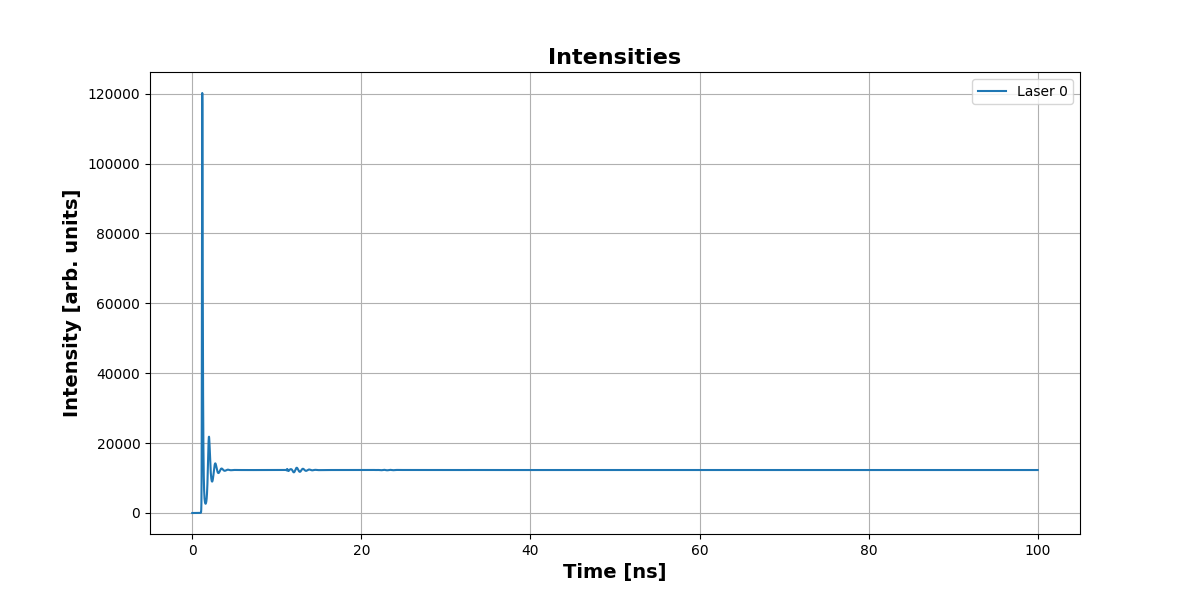
\includegraphics[width=1.0\linewidth]{misc/1laser_0p0012kappa_10ns_18mA_intensity.png}
\caption{Intensity of relaxation oscillation of a single self coupled laser w/ $\kappa = 0.0012$, $\tau = 10$ns, $I_{injection}=18$mA.\label{relaxationosc}}
\end{figure}

\begin{figure}[H]
\centering
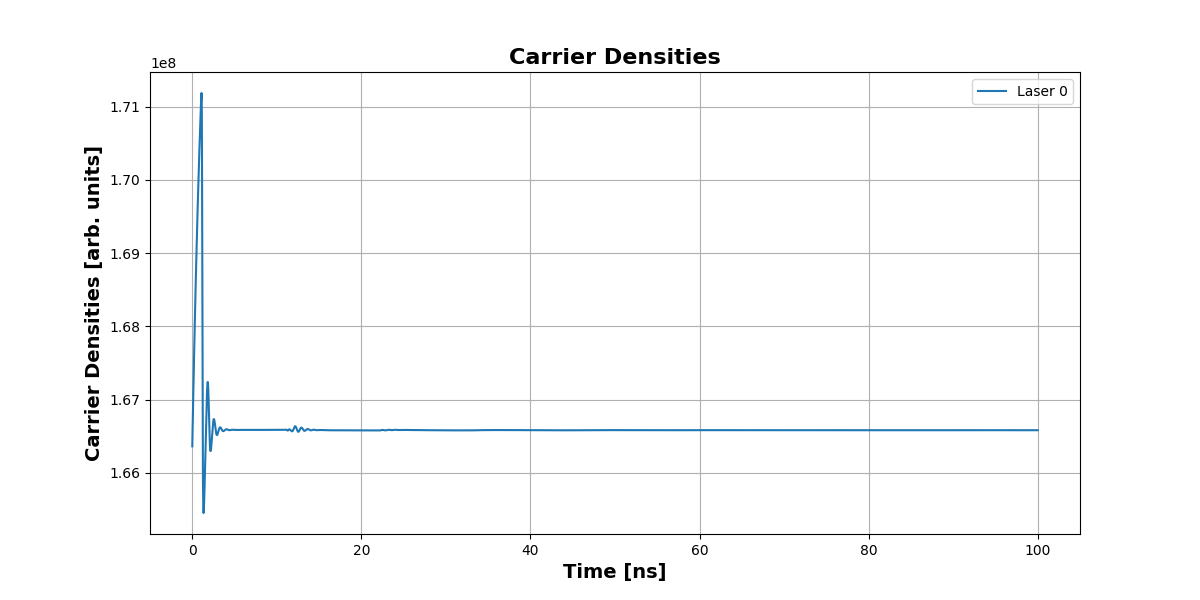
\includegraphics[width=1.0\linewidth]{misc/1laser_0p0012kappa_10ns_18mA_carrierdensity.png}
\caption{Carrier density during relaxation oscillation of a single self coupled laser w/ $\kappa = 0.0012$, $\tau = 10$ns, $I_{injection}=18$mA.\label{carrierdensityrelaxationosc}}
\end{figure}

Also shown here is the carrier density inside the laser. This is something we can measure if needed by measuring the voltage across the laser junction. See Ohtsubo pg. 435 for how voltage relates to carrier density.

Increasing the self-coupling, we now observe chaotic oscillations, shown in Fig.~\ref{chaoticosc}.

\begin{figure}[H]
\centering
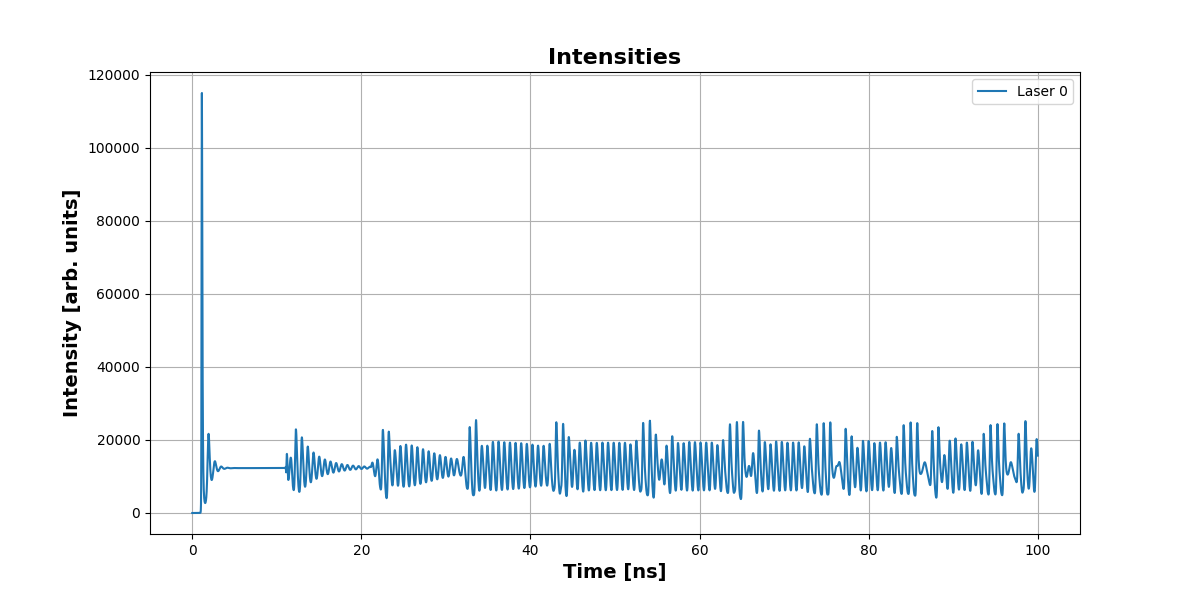
\includegraphics[width=1.0\linewidth]{misc/1laser_0p012kappa_10ns_18mA_intensity.png}
\caption{Relaxation oscillation of a single self coupled laser w/ $\kappa = 0.012$, $\tau = 10$ns, $I_{injection}=18$mA.\label{chaoticosc}}
\end{figure}

Further increasing the self-coupling, and also increasing the injection by a few mA, we can observe periodic oscillations, shown in Fig.~\ref{periodicosc}.

\begin{figure}[H]
\centering
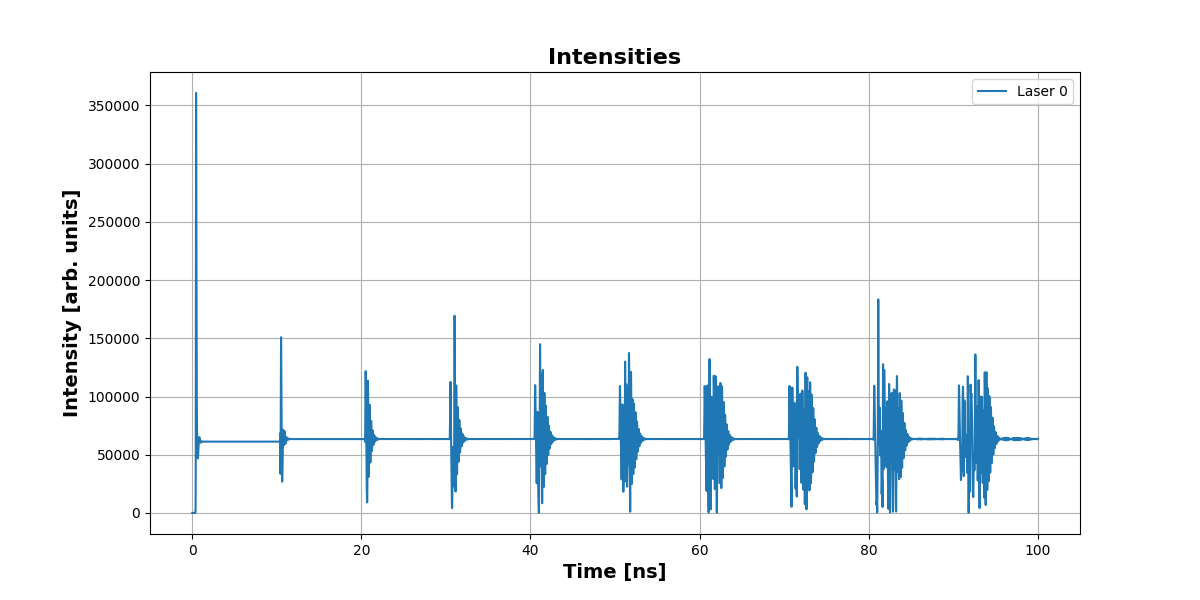
\includegraphics[width=1.0\linewidth]{misc/1laser_0p12kappa_10ns_22mA_intensity.png}
\caption{Relaxation oscillation of a single self coupled laser w/ $\kappa = 0.12$, $\tau = 10$ns, $I_{injection}=22$mA.\label{periodicosc}}
\end{figure}

\subsection{Two Lasers Simulations}

I played around with changing the coupling parameters/delay times for two lasers coupled together. Highly chaotic behavior can be observed; here is an example where laser 0 is coupled to laser 1 as well as to itself. Both lasers are being driven at their threshold currents. Both lasers oscillate rapidly between on and fully off, shown in Fig.~\ref{twochaoticosc}.

\begin{figure}[H]
\centering
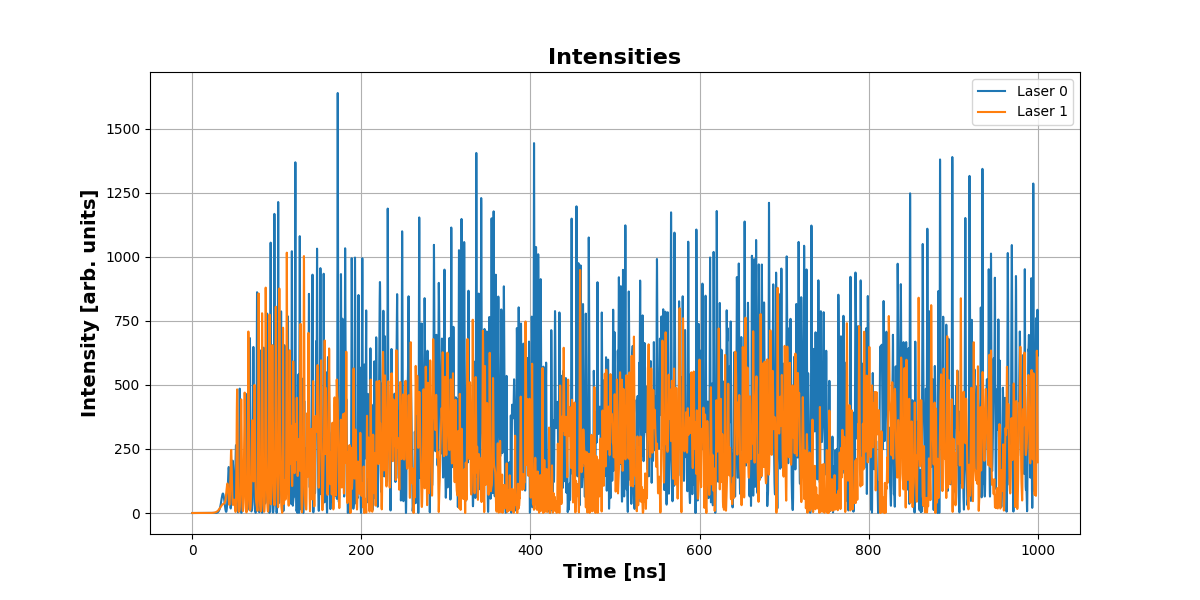
\includegraphics[width=1.0\linewidth]{misc/2laser_0p012kappa_10ns_intercouple_0p012kappa_50ns_l0selfcouple_17mA_intensity.png}
\caption{Highly chaotic oscillations of a two coupled lasers.\label{twochaoticosc}}
\end{figure}

\subsection{Comments}
\begin{itemize}
    \item Want to take the FFT of the chaotic oscillations to see its frequency spectrum
    \item What is the speed of the photodetectors that we can build on-chip? I have read they have a response of 1-10MHz. If it's too slow, we won't be able to see this phenomena.
    \item We could try to induce some kind of low-frequency flucuations (LFF) (see Ohtsubo pg. 140) that would be slow enough detectable. This requires a long delay time. I wonder if we attach a single long fiber optic cable, to a system containing multiple coupled lasers, if this would offer enough long-term memory.
    \item Next step: add in code a way to be able to change the injection current during the simulation. Right now it is constant.
\end{itemize}

\section{July 14, 2025}

\begin{itemize}
    \item Implemented FFT analysis of intensity vs. time, and a low pass filter on intensities to emulate the limited response speed of a photodetector.
    \item Refactored entire notebook for ease of use
\end{itemize}

\subsection{Thoughts}
\begin{itemize}
    \item We wish to measure a "steady state" laser signal. But for what configurations is there actually a steady state, and for what configurations are there only chaotic oscillations?
    \item Prof. Gmachl says its possible to measure the GHz frequencies by heterodyning two signals at the photodetector (Prof. Wysocki does this).
    \item If the laser is oscillating chaotically on to off, is its average power output lower than it would be if it was outputting at steady state? This average power is a low frequency signal and would be detectable by our photodetectors.
    \item Want to find the intensity vs current curve of a single, uncoupled laser according to the laser equations.
    \item Need an efficient way to simulate many variations on parameters.
    \item Far future: modify the equations to include effect of external light that does not couple into the laser yet still depletes the carrier density in the laser. This is mentioned somewhere in Ohtsubo.
    \item Future work: convert carrier density to voltage, to get an IV curve of a single uncoupled laser
\end{itemize}

\subsection{Coupling Coeffecients}
\subsubsection{Feedback Coefficient $\kappa$}

Assuming the reflectivities for the front and back facets are both $r_0$, (see Ohtsubo pg. 87)

\begin{equation}
\kappa = (1-r_0^2)\frac{r}{r_0}
\end{equation}

where $r$ is the external reflection.

\subsubsection{C Parameter for single-laser self-feedback}

\begin{equation}
C = \frac{\kappa \tau}{\tau_{in}} \sqrt{1 + \alpha^2}
\end{equation}

When $C < 1$, the solitary laser is stable and no chaotic oscillations can be observed. (see Ohtsubo pg. 89)

\subsection{Intensity vs Current Curve}

I ran transient simulations with varying injection currents for a single laser with no self-coupling. I capture the value of the intensity at the end of the simulation once it has reached steady state value. As expected according to the theoretical model, the intensity is zero when current is under the threshold current, and increases linearly when current is above the threshold.

\begin{figure}[H]
\centering
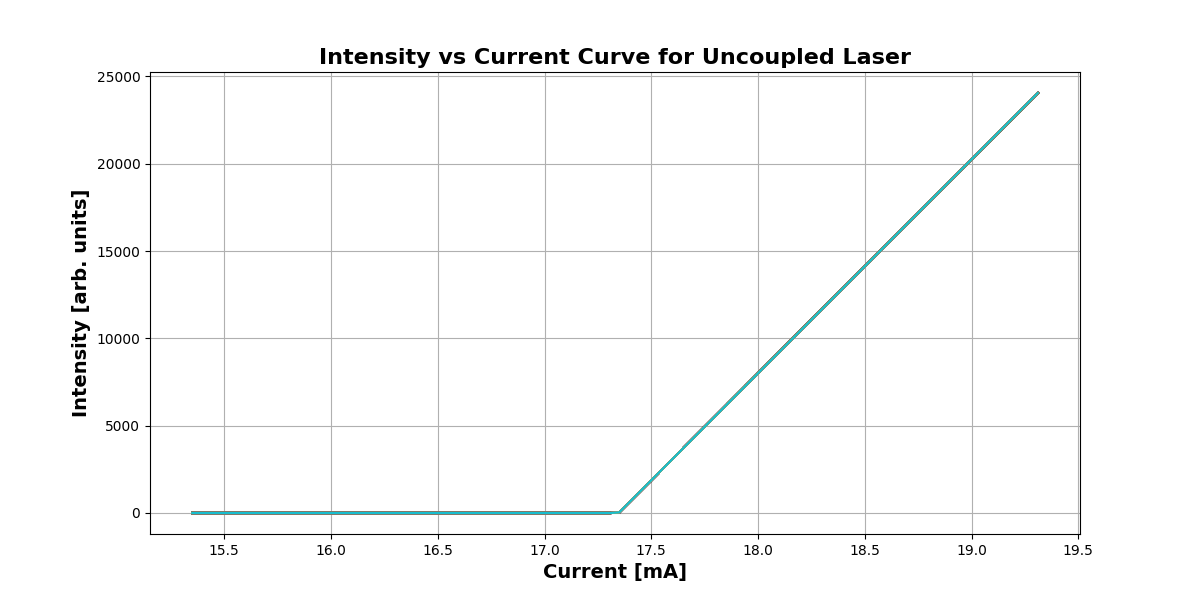
\includegraphics[width=1.0\linewidth]{1laser/experiment3/1laser_uncoupled_intensity_vs_current_fine.png}
\caption{Intensity vs. Current Curve of a single uncoupled laser\label{intensitycurveuncoupled}}
\end{figure}

\section{July 15, 2025}

\subsection{Variable current during simulation}
\subsubsection{Changing parameters}
I add a parameter instead of a constant current for I\textunderscore injection, and when it is time to set a new injection current, I pause the integration, change the parameter, and resume integration.

If no discontinuity smoothing is done after the change, sometimes the integrator fails to solve the system. On the other hand, if step\textunderscore on\textunderscore discontinuities() or adjust\textunderscore diff() is used after the change, there are huge spikes in the result as seen in~\ref{bigunwantedspikes}.

\begin{figure}[H]
\centering
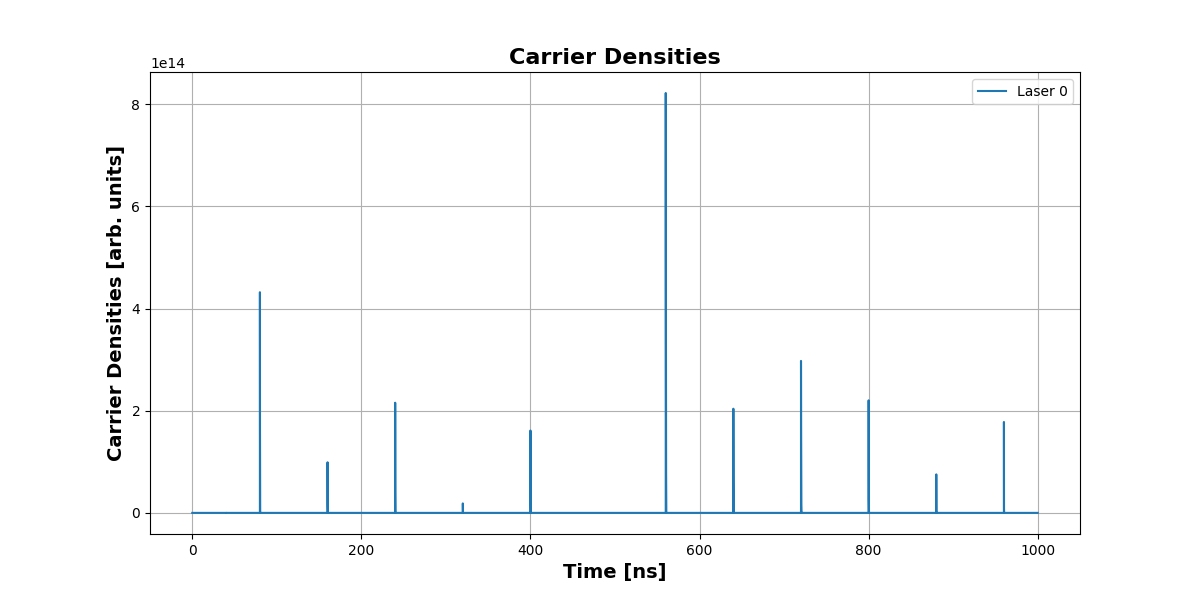
\includegraphics[width=1.0\linewidth]{misc/bigunwantedspikes.png}
\caption{Huge spikes due to discontinuous injection current changes.\label{bigunwantedspikes}}
\end{figure}

\subsubsection{Smoothed current changes}
I coded an alternate simulation method, not using the parameter changing method, but instead using the continuous function ``conditional". It resulted in smaller spikes but was extraordinarily slow. This was only for 1 laser, so having this for a system of say 100 lasers would be impossible.

So, I went back to the parameter-changing method and fixed the ``shift\textunderscore ratio" parameter to a much larger value (now equal to 1), which smooths out the discontinuity over a larger area. Now the spikes in carrier density are much more tolerable, almost not noticeable. Increasing ``shift\textunderscore ratio" did not have a noticeable effect on the intensity.

\begin{figure}[H]
\centering
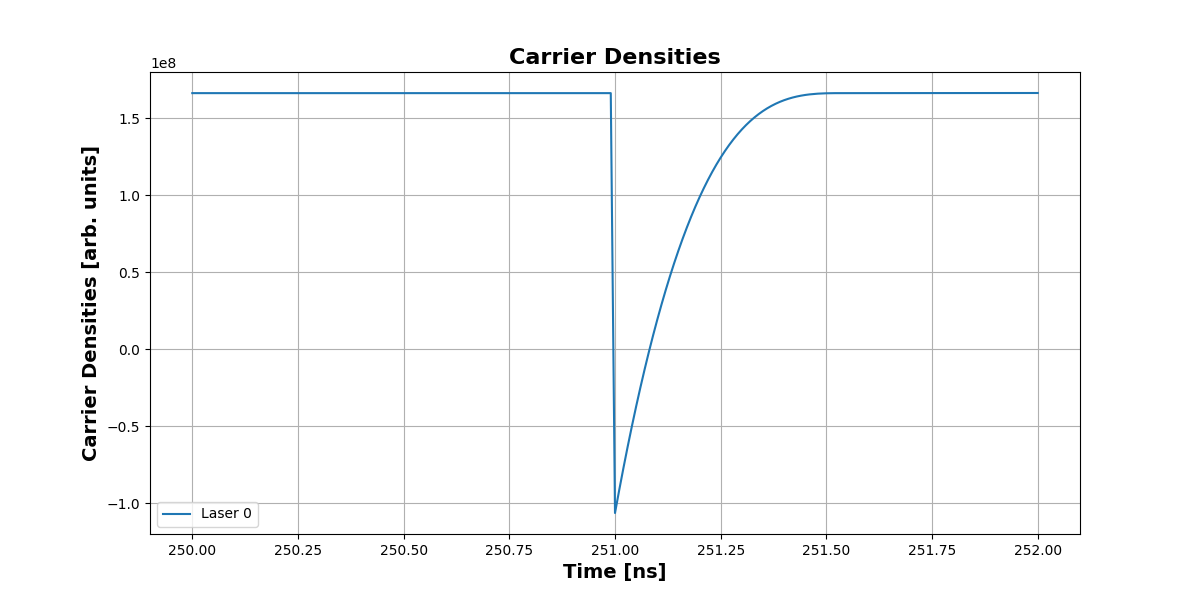
\includegraphics[width=1.0\linewidth]{1laser/experiment4/1laser_switched_fast_0p01shiftratio_0kappa_0ns_threshold_carrierdensity.png}
\caption{Carrier density after a injection current change with ``shift\textunderscore ratio" = 0.01}
\end{figure}

\begin{figure}[H]
\centering
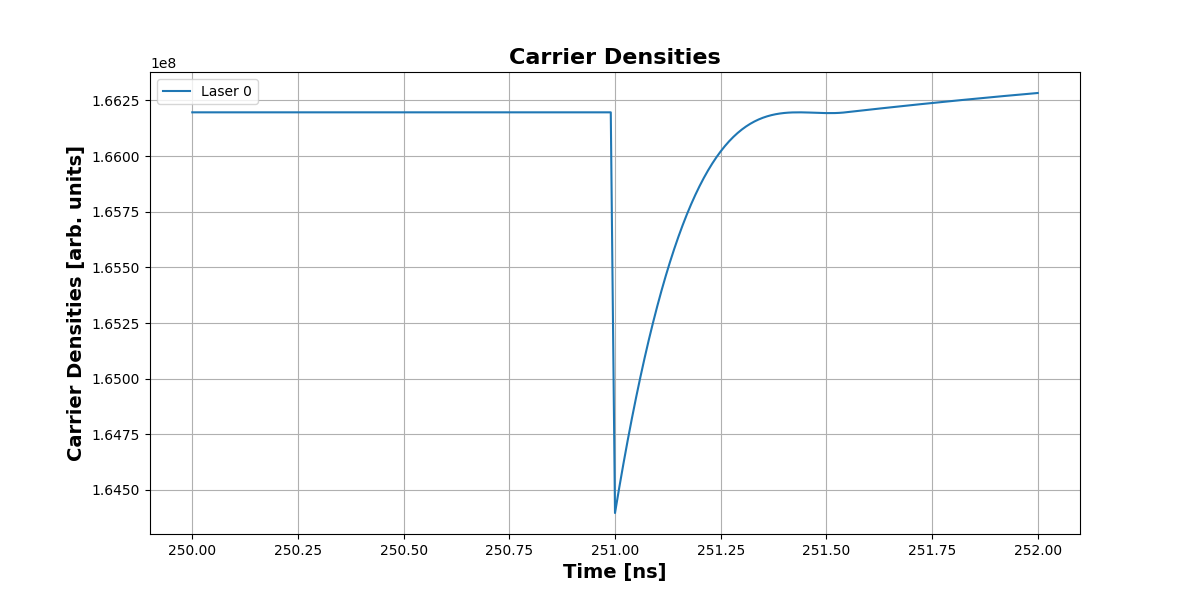
\includegraphics[width=1.0\linewidth]{1laser/experiment4/1laser_switched_fast_0p1shiftratio_0kappa_0ns_threshold_carrierdensity.png}
\caption{Carrier density after a injection current change with ``shift\textunderscore ratio" = 0.1}
\end{figure}

\begin{figure}[H]
\centering
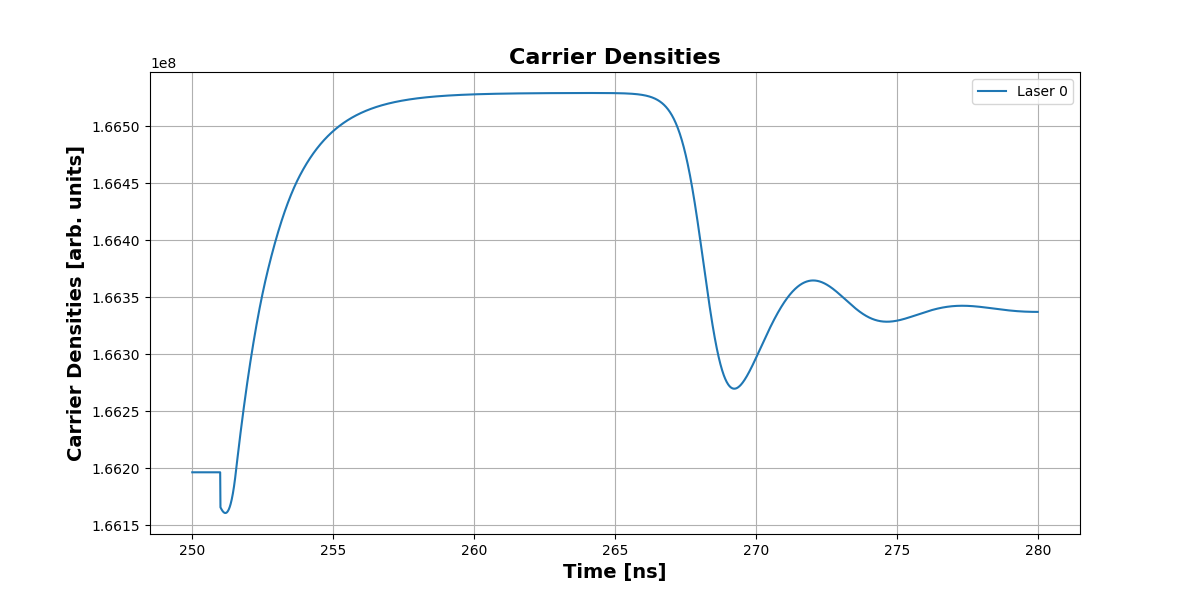
\includegraphics[width=1.0\linewidth]{1laser/experiment4/1laser_switched_fast_1shiftratio_0kappa_0ns_threshold_carrierdensity.png}
\caption{Carrier density after a injection current change with ``shift\textunderscore ratio" = 1}
\end{figure}

\bibliography{main} 

\end{document}